\documentclass{article}

% if you need to pass options to natbib, use, e.g.:
%     \PassOptionsToPackage{numbers, compress}{natbib}
% before loading neurips_2019

% ready for submission
% \usepackage{neurips_2019}

% to compile a preprint version, e.g., for submission to arXiv, add add the
% [preprint] option:
\usepackage[preprint]{neurips_2019}
\bibliographystyle{unsrt}

% to compile a camera-ready version, add the [final] option, e.g.:
%     \usepackage[final]{neurips_2019}

% to avoid loading the natbib package, add option nonatbibnatbib:
%     \usepackage[nonatbib]{neurips_2019}

\usepackage[utf8]{inputenc} % allow utf-8 input
\usepackage[T1]{fontenc}    % use 8-bit T1 fonts
\usepackage{hyperref}       % hyperlinks
\usepackage{url}            % simple URL typesetting
\usepackage{booktabs}       % professional-quality tables
\usepackage{amsfonts}       % blackboard math symbols
\usepackage{nicefrac}       % compact symbols for 1/2, etc.
\usepackage{microtype}      % microtypography
\usepackage{graphicx}
\usepackage{titlesec}
\usepackage{hyperref}
\usepackage{enumitem}
\usepackage{lmodern}
\usepackage{amsmath}
\usepackage{fancyhdr}
\usepackage{textcomp}
\usepackage{lmodern}% http://ctan.org/pkg/lm
\usepackage[table,x11names,svgnames]{xcolor}
\usepackage{soul}
\usepackage{parskip}
\usepackage{multirow}
\usepackage{array}
\usepackage{afterpage}
\usepackage{tabularx}
\usepackage{float}
\usepackage{placeins}
\usepackage{tablefootnote}
\usepackage{microtype}
\usepackage{textcomp}
\usepackage{titlesec}
\usepackage{enumitem}
\usepackage{listings}
\usepackage{subcaption}
\usepackage{verbatim}
\usepackage[htt]{hyphenat}
\usepackage[linesnumbered, noline, noend]{algorithm2e}

% optimization
\DeclareMathOperator*{\argmin}{arg\,min}
\DeclareMathOperator*{\argmax}{arg\,max}


\title{Learn to play Go}

\author{%
  Albert Liu \\
  Department of Computer Science\\
  Stanford University\\
  \texttt{albertpl@stanford.edu} \\
}

\begin{document}

\maketitle

\section{Infrastructure}
As illustrated in Figure \ref{fig:env}, our simulator includes a Go gameplay engine, which is based on Pachi \cite{baudivs2011pachi}, an open source Go framework. We choose Pachi mainly because of the optimized gameplay time. For each player, the input is a 2D numpy array (e.g. $9 \times 9$), representing current board with each element encoding the color of stone, 0 for empty, 1 for black stone and 2 for white stone. The output of each player is the next move to play, which is a scalar that either represents encoded board position (e.g. 50 represents "E4") or a pass action (e.g. 81). Each player can optionally persist the game records, i.e. numpy arrays that hold the board representation, moves and etc., to disk, which are used as experiences for further reinforcement learning. We use Keras as our deep learning framework. 

\section{Approach}
We restrict our attention to $9 \times 9$ board because of resources limitation. Even with such restriction,  the search space is still enormous and therefore Minimax search or AlphaBeta pruning is intractable. Instead, we start with Monte Carlo Tree Search \cite{coulom2006efficient}. Then we will explore policy gradient based methods. Finally we will combine tree search and function approximation approach, following AlphaGoZero \cite{silver2017masteringalphagozero}.  But first, we discuss the baseline and oracle.

\subsection{Baseline}
For baseline, we write a random player which selects legal move randomly, except that it won't commit suicide, i.e. filling in its own eye, which is an empty position where all adjacent positions and three out of four diagonally adjacent positions are its stones (or edges).

\subsection{Oracle}
We use Pachi built-in \textit{UCT} engine as our oracle which is said to achieve highest amateur expect level (KGS 7 dan) on $9 \times 9$ board with reasonable hardware, where dan is expert Go ranking, from 1 to 7 (low to high). Technically the \textit{UCT} engine implements RAVE \cite{gelly2007combining}, instead of classic UCT. This engine incorporates lots of heuristics and predefined patterns beyond basic Go rules, e.g. self-atari detector and ladder testing \cite{baudivs2011pachi}.

\subsection{Monte Carlo Tree Search}
\label{sec:mcts}
We apply MCTS approach to the game of Go. Each node of the search tree is a game state, which is tuple of board representation and player to play. And there is an edge between node $s$ and node $s'$ if and only if there exists some move $a$ such that $s' = \text{Succ}(s, a)$, where $\text{Succ}(s,a)$ is function that returns the next game state $s'$, which is the alternated player and a new board produced by playing the move $a$ on the board of $s$. For each  $s, a$, we maintain visit count $n(s,a)$ and value $q(s,a)$. 

When player is asked to make a move, it create a new tree with current game state $s_0$ as the root node. Then the player simulates multiple random games (each is called a rollout) to evaluate the moves. For each rollout, initially it follows tree policy (we use UCB policy) to traverse the tree down and then expands new node once it reaches the leaf of the tree. From the newly expaned node, it will follow a rollout policy (we use random policy) to finish the game. The final reward is backed up to all the nodes along the path back to root node. Once all rollouts are done, the player selects the move with the maximum visit counts from the root node. Algorithm below describes this process.

\begin{algorithm} 
  \label{algo:mcts}
  \DontPrintSemicolon
  \caption{MCTS with UCB policy}
  \KwIn{root node $s_0$: current game state}
  \KwIn{$c>0$: parameter to control the degree of exploration}
  \While {within computation bound} {
    $ s \gets s_0 $ \\
    $ \Delta \gets \emptyset$ \\
    // selection based on tree policy: Upper Bound Confidence \\
    \While {$s$ is in the tree} {
      $a  \gets \argmax \{ q(s, a) + c \sqrt{\frac{\log \sum_{a'}n(s, a')}{n(s,a)}}$ \}\\
      $\Delta \gets \Delta \cup \{(s, a)\}  $ \\
      $s \gets \text{Succ}(s, a) $\\
    }
    expand tree with the new node $s$ \\
    continue the game from $s$ with random policy and let $r$ be the reward \\
    // update each node on the path $s_0 \rightarrow ... \rightarrow s$ \\
    \For {$s, a \in \Delta $ } {
      $ n(s, a) \gets n(s,a) + 1 $ \\
      $ q(s, a) \gets q(s,a) +  \frac{1}{n(s,a)} (r - q(s,a))$ \\
    }
  }
  \Return{$\argmax_{a} q(s_0, a) $}
\end{algorithm}


Figures \ref{fig:mctsselect}, \ref{fig:mctsexpand}, \ref{fig:mctsbackup}, \ref{fig:mctsfinal} show concret examples for each MCTS step.

\subsection{Self-play}
In order to apply reinforcement learning, we need to collect experiences (i.e. game records). The standard approach is to have player play against themselves and save the game records. We record the board position at each step perceived by the player, the move of the player, the color of the player, the final reward (-1 if white player wins, +1 if black player wins) and network predictions. Then later the player can use these experiences to update its network.

\subsection{REINFORCE with baseline}
The policy gradient based methods, such as REINFORCEMENT \cite{williams1987reinforcement}, allow us to learn stochastic policy naturally, compared to using $\epsilon-$ greedy policy in Q-learning. REINFORCE method uses Monte Carlo method to sample return to compute an unbiased estimation of the gradient. But typically Monte Carlo methods have high variance and therefore produces slow learning. An extra baseline term, as suggested in \cite{sutton2018reinforcement}, can greatly reduce the variance without any bias, because the added term has an expectation of zero. We now describe how we apply this method in this problem.


\subsubsection{Network architecture}
\label{sec:nn}
Let $t$ be current move index of current player, $S_t$ be state the player makes decision on and $A_t$ be move the player will take. As shown in Figure \ref{fig:nn}, we have a two headed deep neural network to approximate both the policy function $\pi_{\theta}(A_t|S_t)$ and state value function $v_w(S_t)$.  The input to this network is $S_t$, which is an array in the shape of $17 \times 9 \times 9$, where $9$ is the board size and $17$ is the number of channels and each channel is described as following 

\begin{enumerate}
  \item
    For $i = 0, ..., 7$, channel $i$ is a $9 \times 9$ 2D array and each element is an indicator if current player has a stone at the position, at time $t-i$.
  \item
    For $j = 0, ..., 7$, channel $j+8$ is a $9 \times 9$ 2D array and each element is an indicator if opponent player has a stone at the position, at time $t-j$.
  \item
    The last channel ($16$) encodes current player, 1 for black player and 2 for white player.
\end{enumerate}

The outputs of the network are 
\begin{itemize}
  \item
    $\pi_{\theta} (A_t|S_t)$

    A $82$-tuple of representing the probability vector for taking each action $A_t$ for $S_t$ for current player. The action space size is $9 ^2 + 1 = 82$.

  \item
    $v_w(S_t)$

    A scalar between -1 and +1, representing the predicated value for $S_t$, from the perspective of current player.

    Figure \ref{fig:inference} shows an sample input/output for the neural network.
\end{itemize}

$\theta$ and $w$ share most of the parameters (ResNet and two Fully Connected layers), except that $\theta$ includes a Softmax layer and $w$ includes a Tanh layer.


\subsubsection{Training procedure}
We set the reward to +1 if current player wins, -1 if loses. No reward otherwise. 

Let $\alpha$ be the learning rate,  $G_t$ be return. Let $s_t, a_t, r_t$ be specific training sample, representing player taking action $a_t$ at state $s_t$ and yielding final reward $r_t$.

For policy function and $\theta$. The objective function is  $J(\theta) = V_{\pi_{\theta}}(S_t)$ and update rule is
$$ \theta_{t+1} = \theta_{t} + \alpha 
( r_t  - v_w(s_t))
\nabla_{\theta} \log \pi_{\theta}(a_t|s_t) 
$$

For value function and $w$. The objective function is  $J(w) = ||v_w(S_t) - G_t||^2$ and update rule is 
$$ w_{t+1} = w_{t} + \alpha 
( r_t  - v_w(s_t))
\nabla_{w} v_w(s_t) 
$$
\subsection{Tree Search guided with NN}
Finally we will apply similar approach as in AlphaGoZero \cite{silver2017masteringalphagozero}, which combines MCTS and function approximation by NN. This method can be viewed as an general form of policy iteration \cite{sutton2018reinforcement}. Assume we reuse the same network, as described in \ref{sec:nn}. We repeat the following two steps until it converges

\begin{itemize}
  \item
    Tree search

    We use same MCTS,  with variations, during self play to gather experiences. Let $s$ and $a$ follow the same definition as in \ref{sec:mcts}. Whenever we expand a new node $s$, instead of play out the rest of the game to estimate the value, we perform an inference over $s$ and use $v_w(s)$ as our estimation of the final reward. Also we add a prior distribution $\pi_{\theta}(a|s)$ to the UCB rule,
$$a  \gets \argmax \{ q(s, a) + c \pi_{\theta}(a|s) \frac{\sqrt{\sum_{a'}n(s, a')}}{1 + n(s,a)} \}$$
   
Essentially MCTS yields a better policy (than our parameterized policy function $\pi_{\theta}$) and produces a sample of state $s_t$, probability vector $p_{s_t}$ and final reward $r_t$, for every move $t$ in the self play. 


  \item
    NN training
    
    We use experience gathered in self-play as training samples and train with the loss function
    $$ \text{l}(\theta, w) = \sum_i (v_w(s_t) - r_t)^2 - \sum_a p_{s_t, a} \log \pi_{\theta}(a|s_t)  $$
    
    This is a form of policy evaluation, i.e. we ask NN to produce policy and value estimation as close as possible to statistics from the tree search. 

\end{itemize}

\section{Experimental results \& error analysis}
\subsection{Monte Carlo Tree Search}
Table \ref{tbl:mcts} shows our preliminary results for MCTS approach on $9 \times 9$ board. The results are averaged over 1000 games for each opponent and configuration.  
Like any Monte Carolo method, the accuracy for value estimation of each game state in MCTS is dependent on the number of rollouts. And therefore it is crucial to minimize the run time for each rollout. So we report median run time per game, on top of win rate (number of games MCTS wins / number of total games) and number of rollouts per move. 

\begin{table}[h]
  \caption{Results of 1000 games between MCTS and opponents on $9 \times 9$ board, no Komi, MCTS plays first}
  \label{tbl:mcts}
  \centering
  \begin{tabular}{c | c | c | c}
    opponent policy    &  number of rollouts per move & win rate  & median time per game \\
    \hline
    random            &  100 &  0.92  & 2.4 \\
    random            &  1000 &  0.99  & 29.3 \\
    pachi \textit{UCT} engine  &  1000 &  0.16  & 35.1 \\
  \end{tabular}
\end{table}


We see MCTS win rate gets better with more rollouts per move, as expected. But it still loses more games against pachi \textit{UCT} engine. And we speculate that reasons are
\begin{itemize}
  \item
    Rollout policy 

    Unlike our MCTS, pachi entails more Go knowledge when selecting next move during the game simulation. This is called \textbf{heavy} or strong rollout policy, whereas ours is light rollout policy, i.e. no heuristics other than not filling eyes. Pachi's rule based simulation policy is handcrafted to mix in heuristics such as,  if the last move has put its own group in \textit{atari} we capture it; \textit{Nakade}a move is played inside the eyeshape to prevent the opponent from splitting it into two eyes \cite{baudivs2011pachi}.

  \item
    Priors
  
    We expand a new node by randomly selecting a legal move. But Pachi apply again a set of heuristic function to this decision, equivalently adding a prior probability distribution.  Specifically it takes the progressive bias strategy \cite{gelly2007combining}, which adds virtual simulations based on the applied heuristics with decreasing weights as the nodes are explored.

  \item
    RAVE 

    MCTS updates values of nodes with the reward of the simulation, along the sampled path from root to the leaf. But RAVE \cite{gelly2007combining} distributes the update to larger set of nodes. Basically it applies AMAF heuristics \cite{bouzy2004monte} (all-move-as-first), which keep previous simulations and apply it whenever we examine the same $(s, a)$ edge and then combines it with regular simulations.
\end{itemize}


    We believe the REINFORCE with baseline and the tree search guided by NN are a better approaches and therefore didn't engage any of these improvements yet.  But both of those approaches are under development and we are not ready to report any results yet. 


\bibliography{reference} 

\newpage

\section{Appendix}
\subsection{Figures}
\begin{figure}
\centering
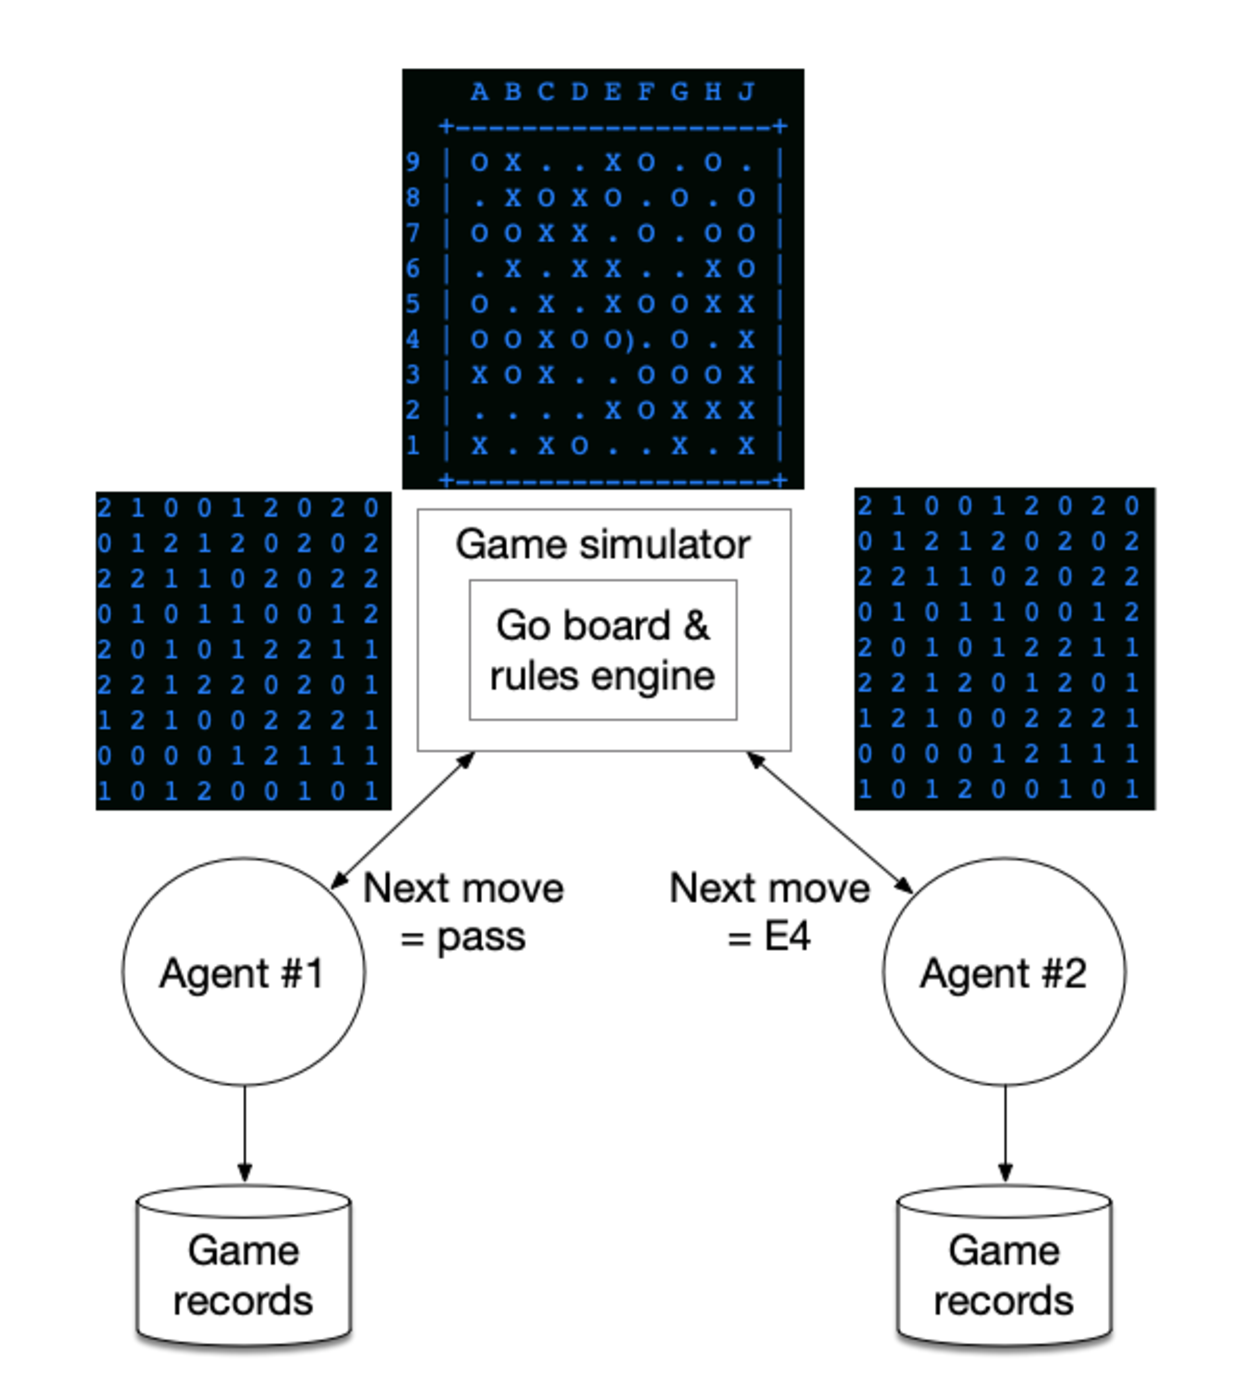
\includegraphics[width=0.8\linewidth]{simulator}
\caption{Environment setup. For Go boards drawn in all the figures, 'x' represents black stone and 'o' represents white stone. For numpy arrays, '0' means empty, '1' represent black stone and '2' represents white stone. All examples assume $9 \times 9$ board.}
\label{fig:env}
\end{figure}

\begin{figure}
\centering
\includegraphics[width=1.0\linewidth]{mctsselect}
\caption{MCTS node selection via tree policy: shows 4 successor states only for brevity. $a=67$ is selected. $n, q$ is visit count and value for each node respectively. $a=76$ has more visit counts but lower value.}
\label{fig:mctsselect}
\end{figure}

\begin{figure}
\centering
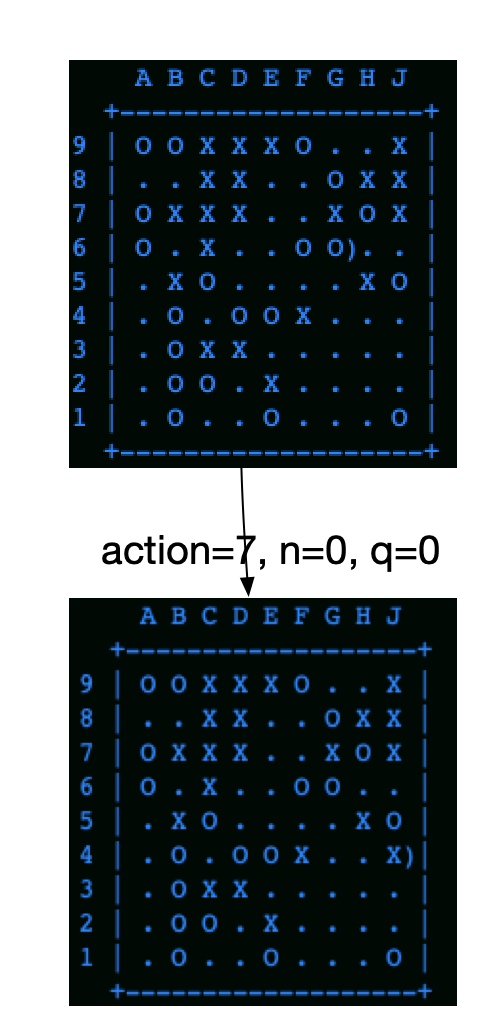
\includegraphics[width=0.3\linewidth]{mctsexpand}
\caption{A new node $\text{Succ}(s, a=7)$, randomly chosen, is expanded with zero visit count and value. }
\label{fig:mctsexpand}
\end{figure}

\begin{figure}
\centering
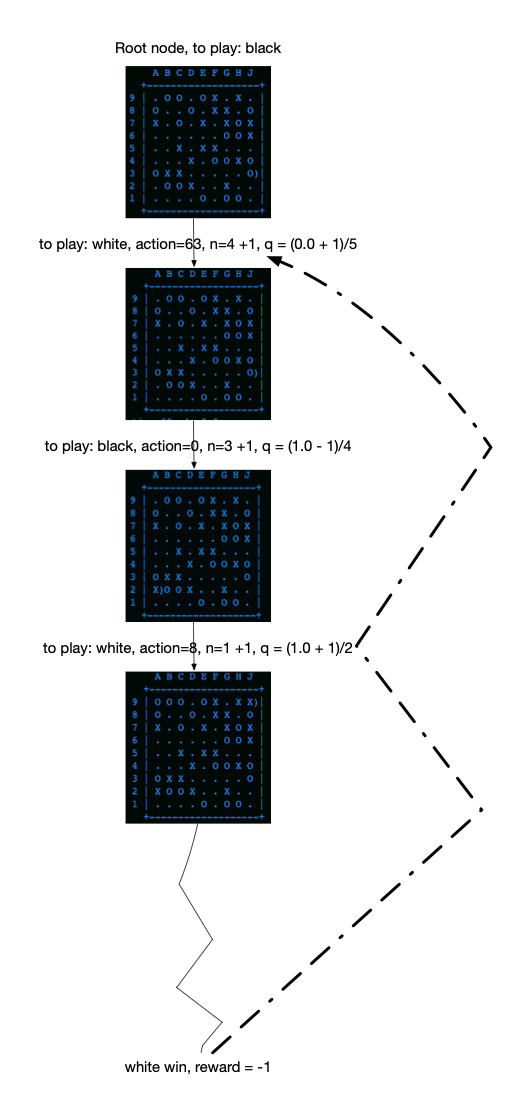
\includegraphics[width=0.7\linewidth]{mctsbackup}
\caption{After the simulation is done. The result is backed up to all nodes on the path. Note the reward is from black player's perspective and needs to be adjusted for white player.}
\label{fig:mctsbackup}

\end{figure}
\begin{figure}
\centering
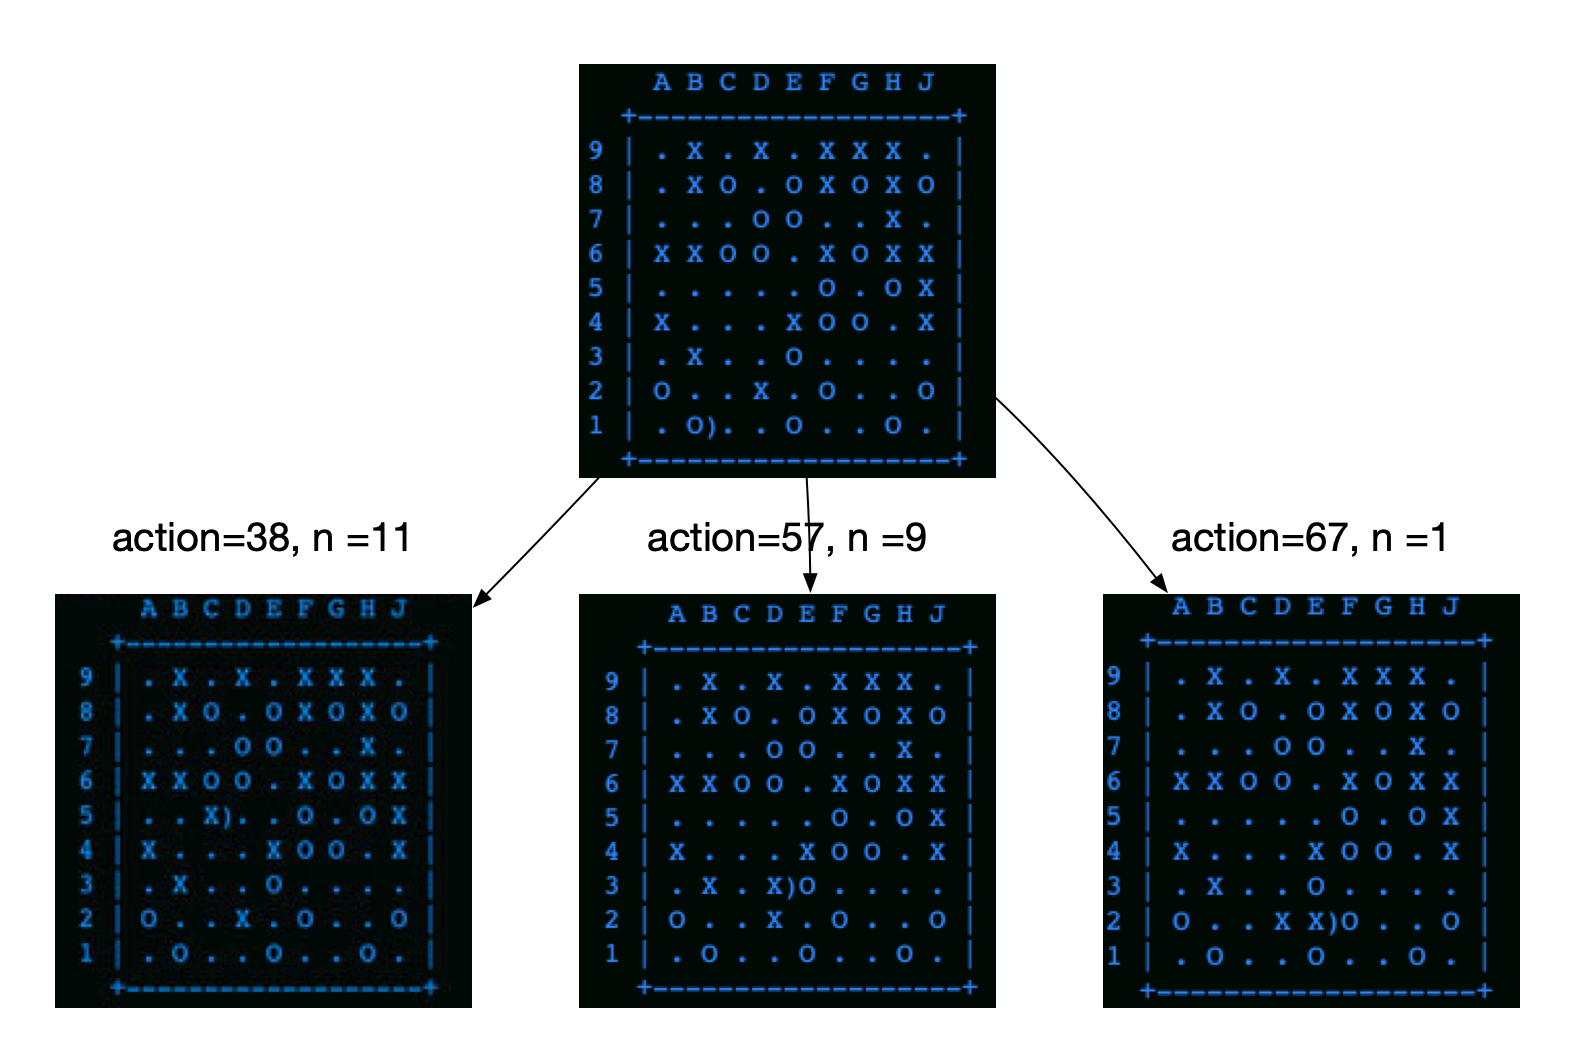
\includegraphics[width=0.9\linewidth]{mctsfinal}
\caption{After all rollout are done. Select the next move with maximum moves. Shows 3 successor states from root state only. The action $a=38$ is selected.}
\label{fig:mctsfinal}
\end{figure}

\begin{figure}
\centering
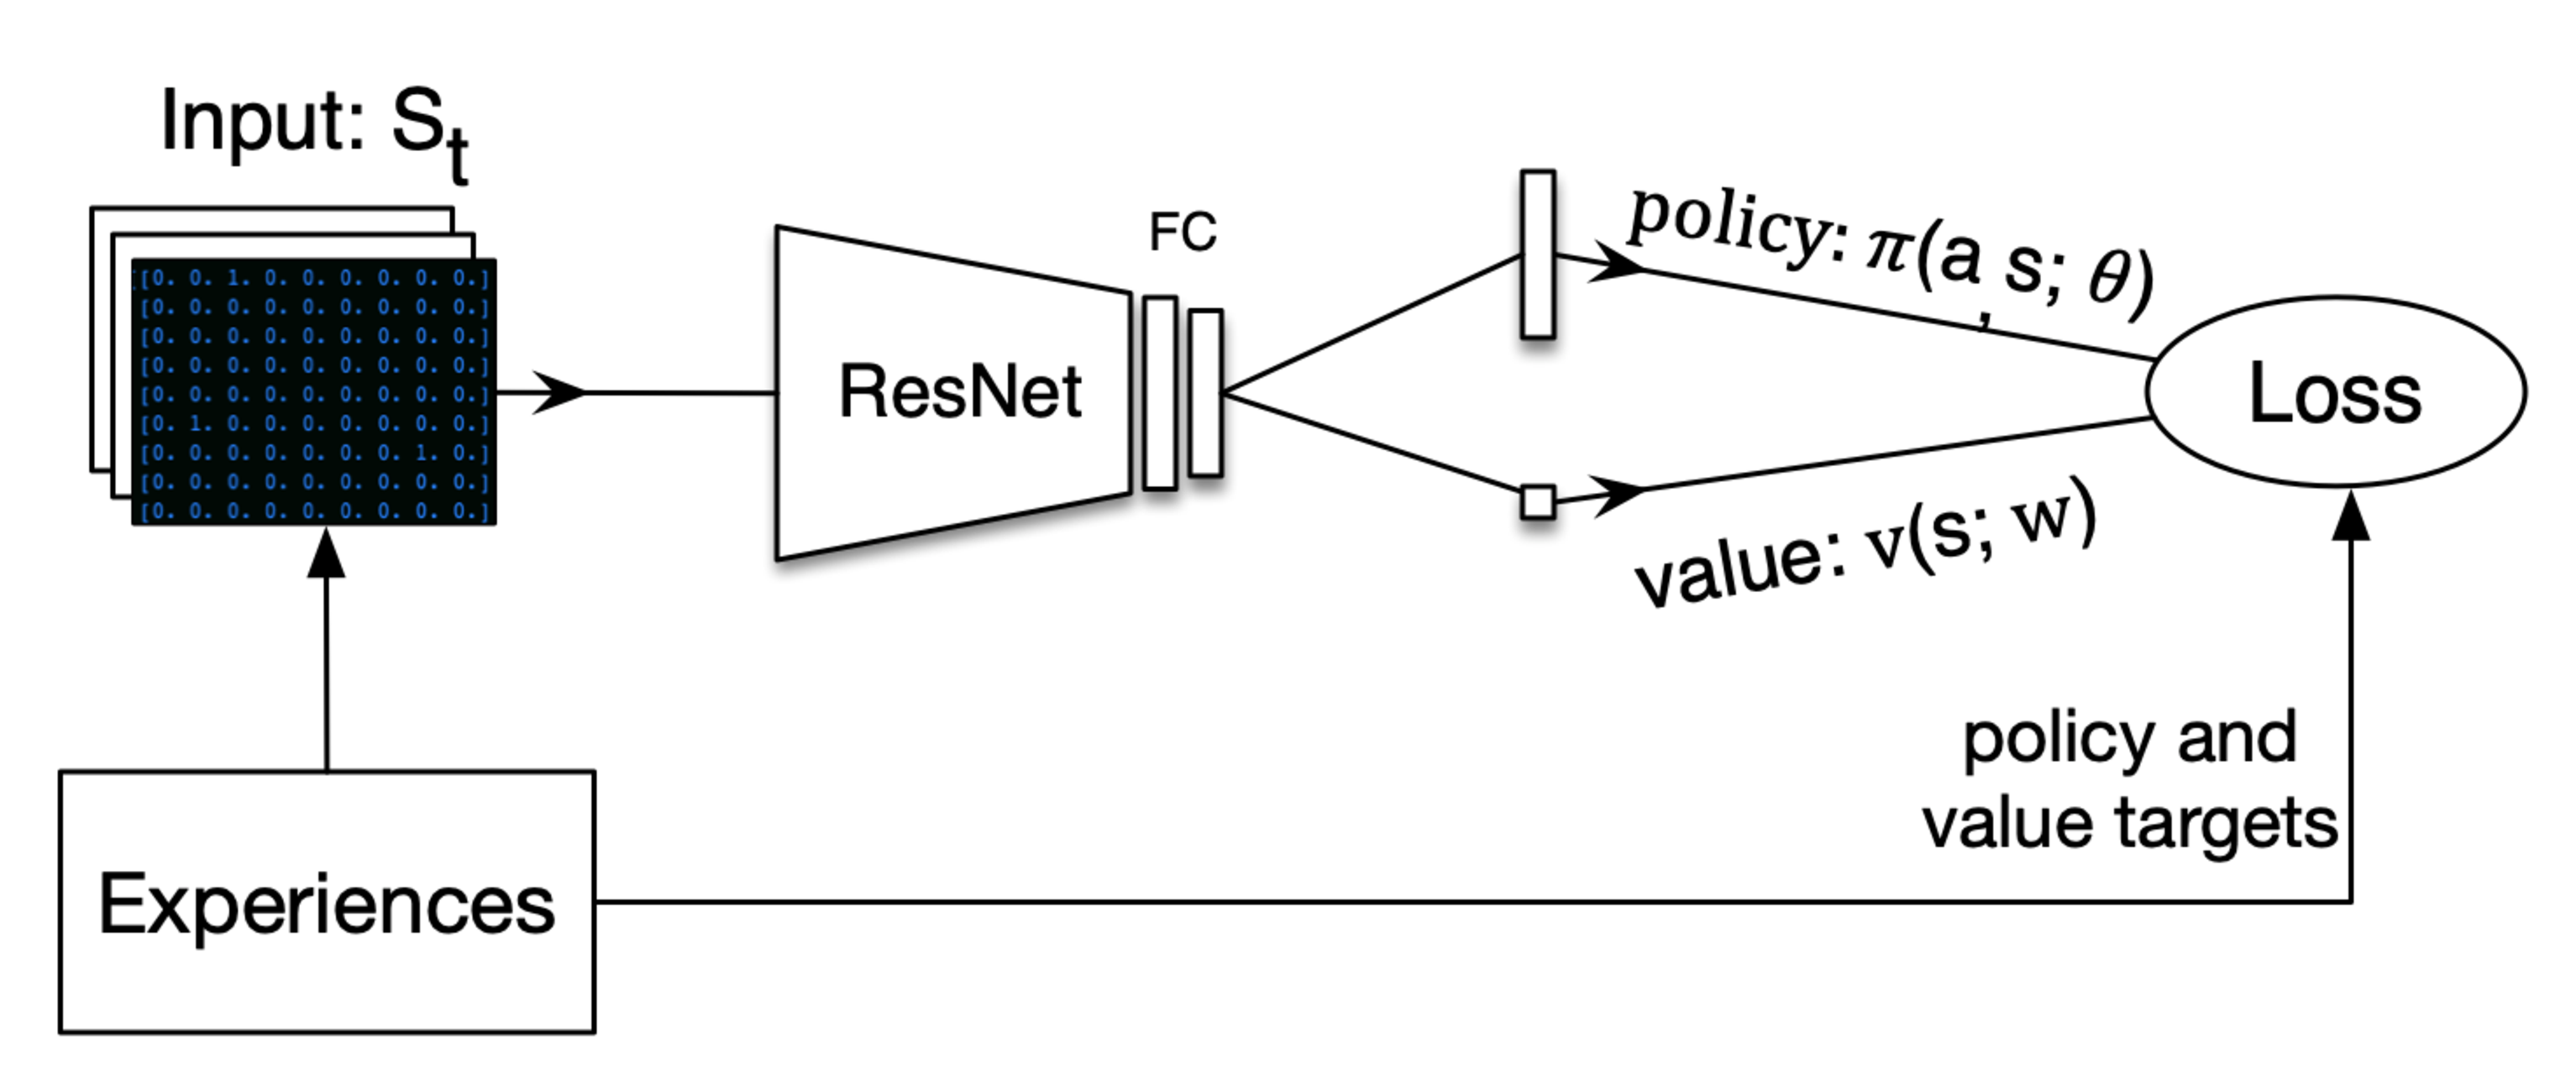
\includegraphics[width=0.8\linewidth]{nn}
\caption{network architecture for policy gradients and NN guided MCTS approaches. The features and policy/value targets are gathered from self-play experiences. FC stands for Fully Connected layer. Features, targets and Loss are discussed in details in text.}
\label{fig:nn}
\end{figure}

\begin{figure}
\centering
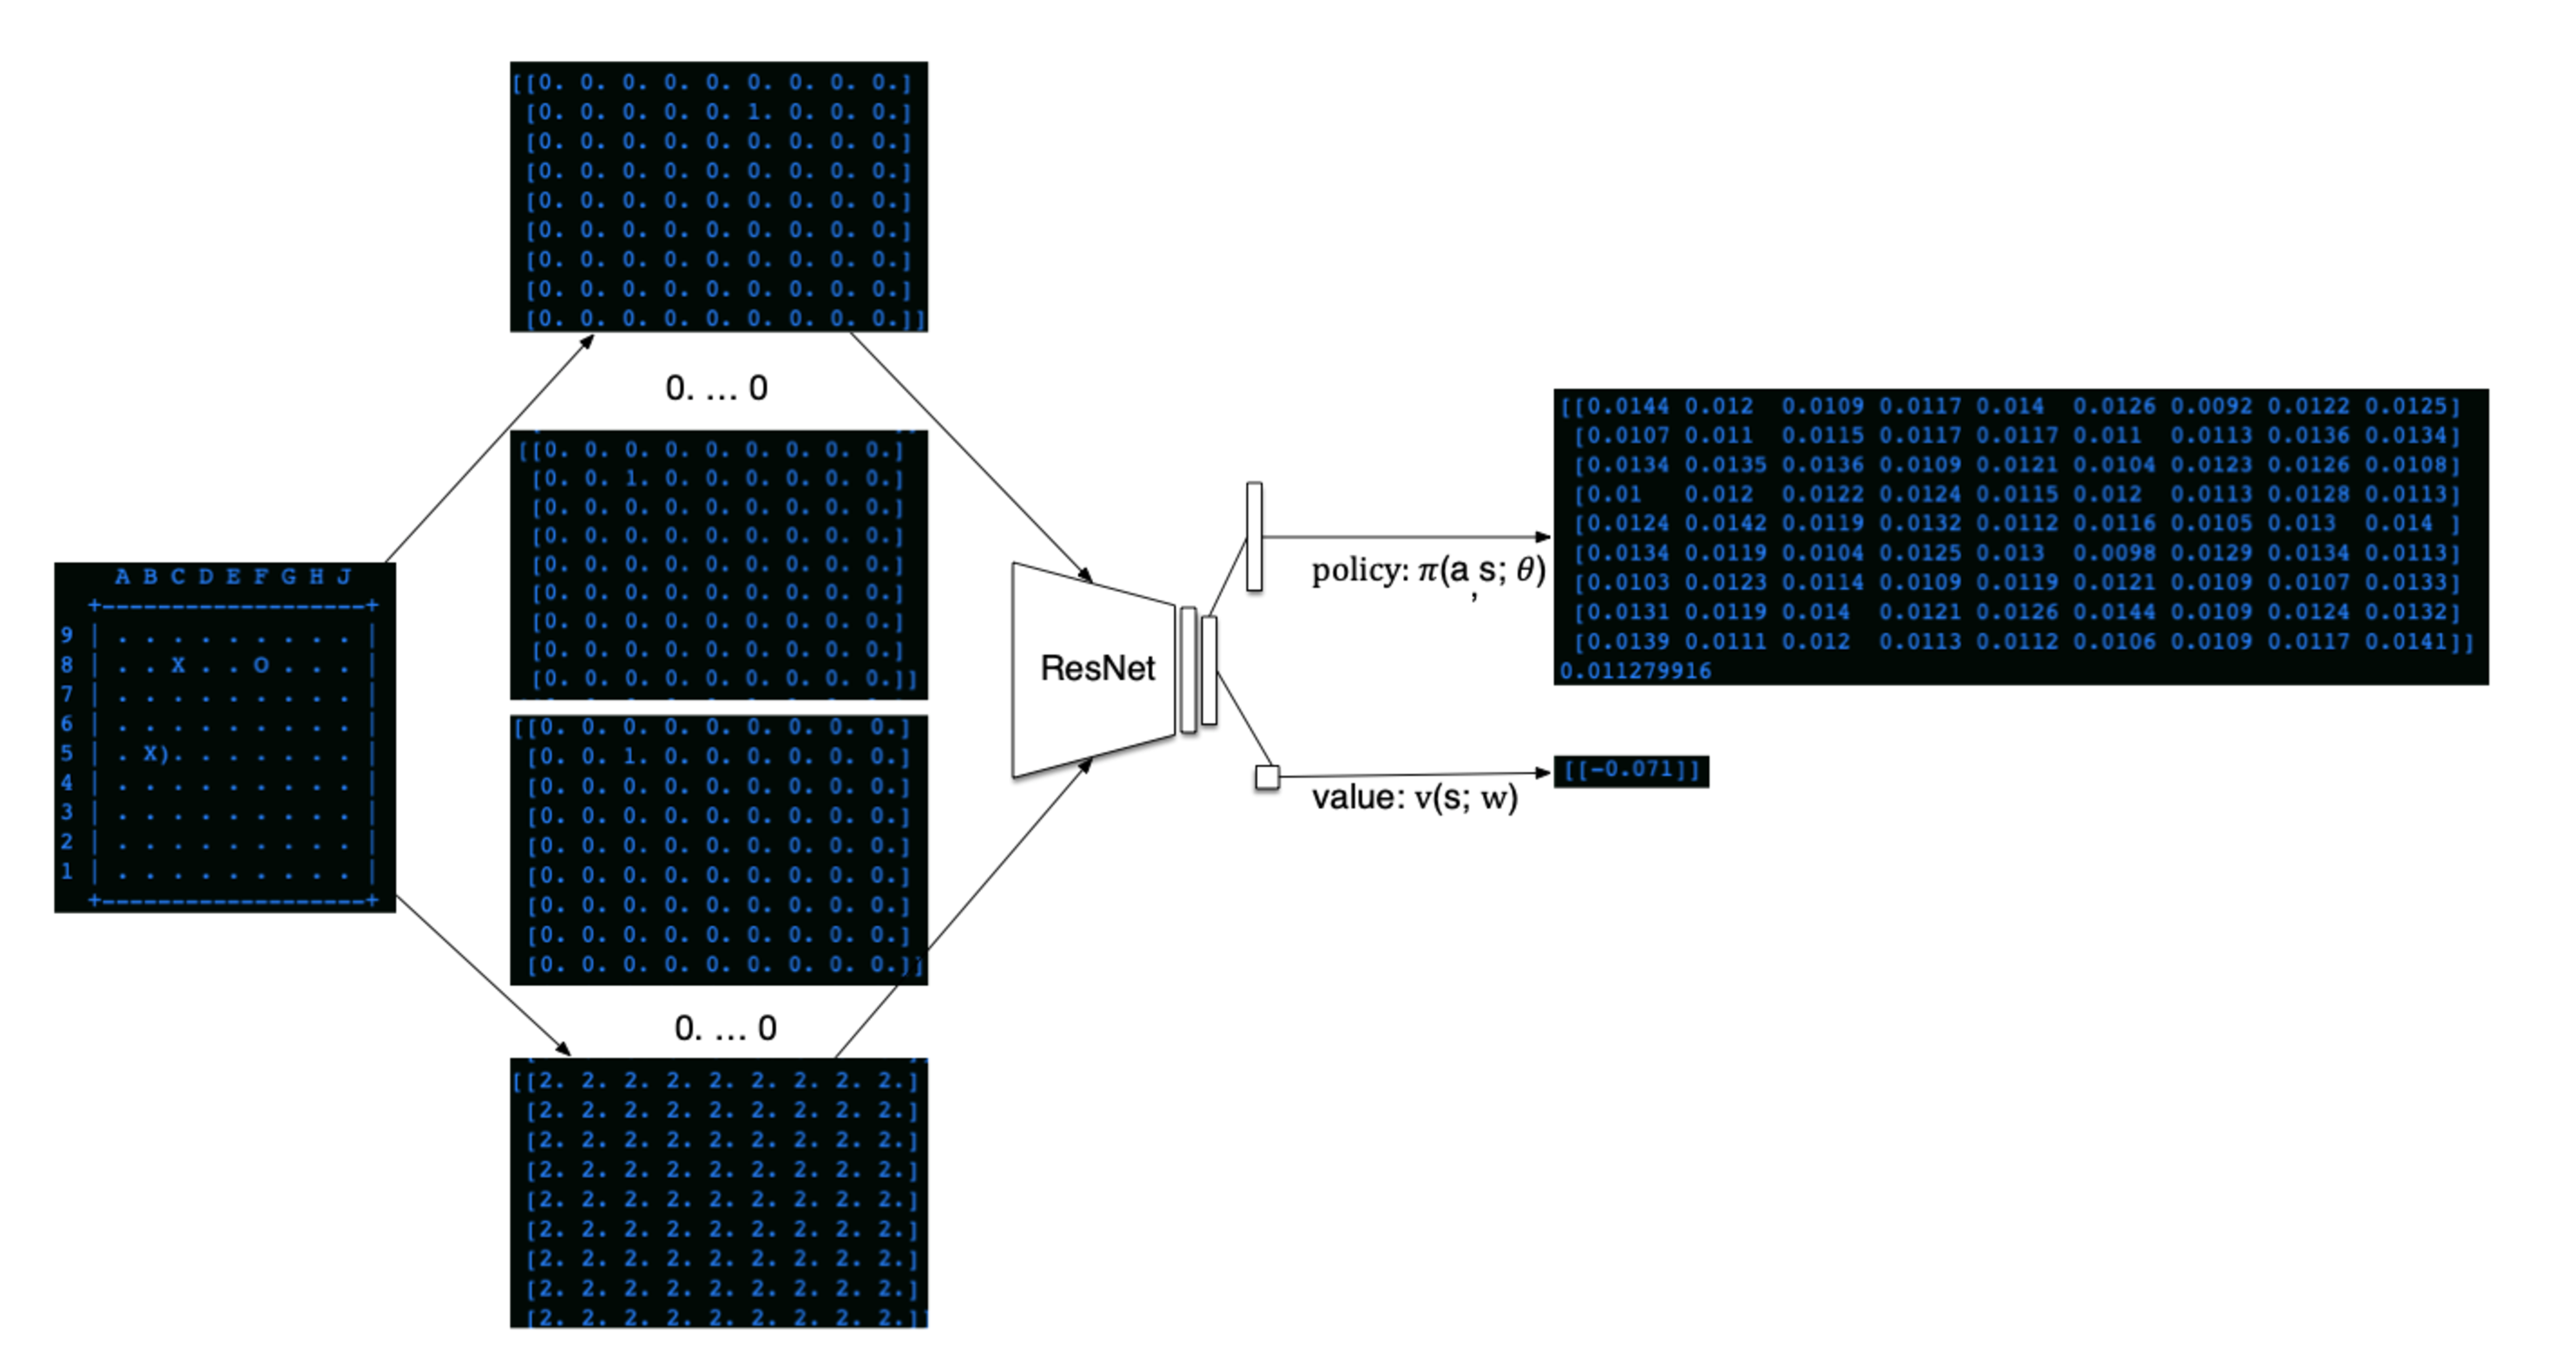
\includegraphics[width=1.0\linewidth]{inference}
\caption{example for an input/output for neural network. The input is $17 \times 9 \times 9 $ arrays, created from the board position. There are two outputs, one $82$-tuple of probability vector $\pi_{\theta}$ and one scalar $v_w \in [-1, 1]$. Refer to the text for more details. }
\label{fig:inference}
\end{figure}

\end{document}
